\begin{frame}
  \frametitle{The Problem: Minimal Bi-Partitional RatioCut}
  \begin{figure}
    \centering
    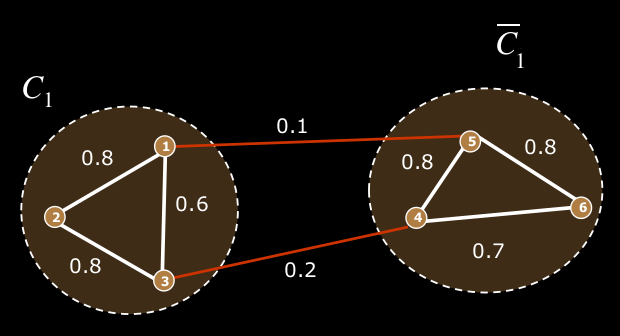
\includegraphics[width=6cm,height=3cm]{min-bip-cut}
  \end{figure}
  \begin{itemize}
  \item Can be seen as an NP-Hard discrete optimization problem (where $G = (V,W)$ is the graph represented by $W$):
    \begin{equation*}
      \min\limits_{\tiny{C_1 \ds{\subset} V}} \ds{}
      \underbrace{      
        \frac{1}{2}
        \left[
          \dfrac{\func{cut}(C_1,\stcomp{C_1})}{\abs{C_1}} +
          \dfrac{\func{cut}(\stcomp{C_1},C_1)}{\abs{\stcomp{C_1}}}
          \right]
        }_{\func{RatioCut(C_1,\stcomp{C_1})}}
      \ds{\suchthat}
      \func{cut}(A,B) = \sum\limits_{\tiny{i \in A \ds{,} j \in B}} w_{ij}
    \end{equation*}
  \end{itemize}
\end{frame}
